\chapter{Evaluation}
\section{Planning\label{sec:score-planning}}
We evaluated the domain-specific planning algorithm described in
\ffref{alg:iw-optimised}, with different subsets of enhancements and different
parameters. We used the \ac{ALE}, with deterministic games
(\verb-repeat_action_probability=0-). Our code is based in the one available
from \citet{lipovetzky2015classical}.

Recall that our \ac{IW}(3) only evaluates position for pruning, not
on any other tuple.

\begin{itemize}
  \item $max_{ef}$: maximum nodes emulated per frame.
  \item $\gamma$: The discount factor.
  \item $n_a$: number of actions to take without re-planning.
  \item $p_r$: probability that a room is pruned. Blank means zero.
  \item \textit{FS}: frame skip, the amount of frames each action is taken for.
  \item \textit{TR}: Whether the search tree is reused, or the nodes are
    re-emulated in every frame.
  \item Frontier: the data structure/s used to store the frontier:
    \begin{itemize}
      \item $q$: a single \ac{FIFO} queue, like \ac{BFS} and \ac{IW}.
      \item $q,q_l$: two \ac{FIFO} queues, one with a lower priority.
      \item P. Dist.: Priority queue that prioritises nodes more distant (in
        game coordinates, Euclidean distance) to the root.
      \item 2BFS Two priority queues: one prioritising low novelty, breaking
        turns by largest accumulated return, and one prioritising large
accumulated return, breaking ties by lowest novelty \citep{lipovetzky2015classical}.
    \end{itemize}
    \ac{FIFO} queue, 2 \ac{FIFO} queues, or a priority queue.
  \item \textit{EB}: Exploration Bonus. Whether the agent gains 1 reward on
    exploring a new screen.
  \item \textit{OAV}: Obstacle Algorithm Version. The algorithm that waits for
    obstacles to disappear has some variants. Blank means the absence of such
    thing. Version 1 is the nodes that lead into an obstacle are re-enqueued in
    the frontier. Versions between 1 and 2 are other semi-successful
    modifications of it. Version 2 is the one explained in
Subsections~\ref{subsec:domain-explanation} and~\ref{subsec:implementation-iw}.
  \item \textit{EA}: Extended Action set. Whether the algorithm uses the 18
actions possible with the Atari or the 8 distinct actions in \ac{MR}.
\end{itemize}

Additionally, algorithms with an asterisk (*) receive negative rewards (-5000)
on death. The remaining parameters' values are: $max\_wait=20$, $max\_backtrack=7$.

\begin{table}[hbtp]
  \begin{center}
  \begin{tabular}{c|ccccccccccc|c}
    Name       & $max_{ef}$ & $\gamma$ & $n_a$ & $p_r$ & FS & TR         & Frontier & EB         & OAV & EA         & Score     \\
\hline
    \ac{IW}(1) & 150k       & 0.995    & 1     &       & 5  & \checkmark & $q$      &            &     & \checkmark & 0         \\
    2BFS       & 150k       & 0.995    & 1     &       & 5  & \checkmark & 2BFS     &            &     & \checkmark & 540       \\
    \ac{IW}(3)*  & 150k       & 0.995    & 1     &       & 5  &            & $q$      &            &     &            & 4600      \\
    \ac{IW}(3)*  & $1\,500$k  & 0.995    & 1     &       & 5  &            & P. Dist. &            & 1   &            & $2\,500$  \\
    \ac{IW}(3)*  & 300k       & 0.995    & 1     &       & 5  &            & $q,q_l$  & \checkmark & 1   &            & $5\,600$  \\
  \hline
    \ac{IW}(3)*  & 300k       & 0.995    & 1     &       & 5  &            & $q,q_l$  & \checkmark & 1.1 &            & $8\,000$  \\
    \ac{IW}(3)*  & 150k       & 0.99     & 1     &       & 10 &            & $q,q_l$  & \checkmark & 1.1 &            & $10\,200$ \\
    \ac{IW}(3)*  & 75k        & 0.985    & 1     &       & 10 &            & $q,q_l$  & \checkmark & 1.1 &            & 0         \\
    \ac{IW}(3)*  & 10k        & 0.98     & 1     &       & 20 &            & $q,q_l$  & \checkmark & 1.1 &            & 0         \\
  \hline
    \ac{IW}(3)   & 300k       & 0.995    & 1     &       & 6  &            & $q,q_l$  &            & 1.2 &            & 100       \\
    \ac{IW}(3)   & 300k       & 0.999    & 1     &       & 5  &            & $q,q_l$  &            & 1.2 &            & 500       \\
    \ac{IW}(3)   & 300k       & 0.995    & 1     &       & 5  &            & $q,q_l$  &            & 1.2 &            & $6\,700$  \\
    \ac{IW}(3)   & 300k       & 0.999    & 1     &       & 5  &            & $q,q_l$  & \checkmark & 1.2 &            & $7\,100$  \\
  \hline
    \ac{IW}(3)   & 300k       & 0.999    & 1     & 0.25  & 5  &            & $q,q_l$  & \checkmark & 1.2 &            & $4\,700$  \\
    \ac{IW}(3)   & 300k       & 0.99     & 1     & 0.2   & 5  &            & $q,q_l$  & \checkmark & 1.2 &            & $11\,000$ \\
  \hline
    \ac{IW}(3)   & 300k       & 0.99     & 1     & 0.2   & 5  &            & $q,q_l$  & \checkmark & 2   &            & $13\,600$ \\
    \ac{IW}(3)   & 150k       & 0.99     & 2     & 0.2   & 10 & \checkmark & $q,q_l$  & \checkmark & 2   &            & $14\,500$ \\
    \ac{IW}(3)   & 150k       & 0.995    & 2     & 0.2   & 5  & \checkmark & $q,q_l$  &            & 2   &            & $8\,000$  \\
    \ac{IW}(3)   & 150k       & 0.995    & 2     & 0.2   & 5  & \checkmark & $q,q_l$  & \checkmark & 2   & \checkmark & $7\,800$  \\
    \ac{IW}(3)   & 150k       & 0.999    & 3     & 0.2   & 5  & \checkmark & $q,q_l$  & \checkmark & 2   &            & $14\,900$ \\
\end{tabular}
\end{center}
\caption{The results of different planning algorithm variations}
\end{table}

The algorithm described in \ffref{subsec:domain-explanation} obtains the same
score as the latest one, but it avoids opening the two doors. Instead, it finds
a glitch in the game that allows it to spend the two keys without a door. A video of it is available
\href{https://www.youtube.com/watch?v=KSPYzLE0uy8}{online}. The glitch happens
around \href{https://youtu.be/KSPYzLE0uy8?t=172}{2:52}.

To obtain this massive increase in score, we have heavily tweaked the algorithm to this
game. The strategies employed will likely not generalise to all classes of
problems. Some of them might be useful for games that happen in a 2D
spatial environment, such as pruning on position, waiting for obstacles. The
random room pruning heuristic may also be useful in other problems in the
on-line setting that demand exploring multitudes of similar paths.

%IW(1) geffner
%
%no tree reuse, no exploration bonus
%IW(3) with a big negative reward when dying:  8 screens, 4600 score
%
%IW(3) with no incentives and a priority queue prioritising nodes farther away
%2500 score
%
%IW(3) big negative, with double queue, 9 screens 5600 score
%.995, 30000, sscore 5600
%^ with exploration bonus
%
%exploration bonus:
%
%big negative too
%IW(3) re-enqueuing nodes that run into an obstacle 8000, 300k nodes/frame
%same but .99 discount and 10 frame actions 150k nodes/frame: 10200
%sambe but 15, .985, 10k n/f, 0
%same but 20 , 75k nodes and .98 discount 0
%
%
%Ancestors:
%
%No exploration bonus, no death avoidance
%6 frameskip, .995 -> 100 score
%5 frameskip, .999 -> 500
%5 frameskip, .995 -> 6700
%
%with exploration bonus, .999 -> 7100 score
%
%More than 1 action per frame:
%7500 reward
%
%
%Moreexplore
%no incentives: 2900, incentives 8000
%with 10 and .995: 2500, 2900
%
%noreopen: with screen prune probability
%0.25:, discount .999 : 4700
%.2, discount .99 : 13600 (11015 with old algo)
%
%fs 10, actions no recalc 2: 14500 incentives
%
%no explore but with the good pruning, 2 actions, and teh good navigation :8000
%
%with explore but with 18 actions: 7800
%%
%.999 discount
%14900: good exploration with exploration incentives, calc every 3 actions
%(avoids taking a wrong path)
%

\section{Learning}
We trained agents on the first screen of \acl{MR} using the Sarsa algorithm,
with and without options, and using our shaping function
(\ffref{subsec:shaping-function}).

We used a learning rate $\alpha=0.01$ and a discount rate $\gamma=0.995$. We
also used the \emph{annealing} training technique, which consists in reducing
the $\varepsilon$ for the $\varepsilon$-greedy strategy every episode. When
training without annealing we used $\varepsilon=0.1$, and when training with
annealing we used $\varepsilon=\textsc{Max}(0.7 - 3\cdot 10^{-5} \cdot n_e,
0.1)$, where $n_e$ is the episode number. This encourages extra exploration at
the beginning.

The average reward over time can be seen in Figures \ref{fig:without_options} and
\ref{fig:with_options}. In each of those figures, at the left the reward
including the shaping reward is shown, and at the right the environment reward
alone is shown.

\newcommand{\drawtraining}[2]{
\begin{figure}[p]
\begin{center}
%\includegraphics[width=\textwidth/2- 0.2cm]{img/#1-phi.pdf}
%\includegraphics[width=\textwidth/2- 0.2cm]{img/#1.pdf}
\includegraphics[width=\textwidth]{img/sarsa/#1.pdf}
\end{center}
\caption{#2\label{fig:#1}}
\end{figure}
}

\drawtraining{without_options}{Reward per episode, averaged every 1000
episodes, as the training progresses. No options are used. Blue uses
annealing, red does not. Darker lines, with higher value,
do not include the shaping reward $F(\cdot)$; lighter lines show the reward as
the agent experiences it. $y$ axis is reward, $x$ axis is thousands of
episodes.}
\drawtraining{with_options}{Reward per episode, averaged every 1000
episodes, as the training progresses. Options are used. Meaning of each element is
the same as in \ffref{fig:without_options}. Note that the two reward lines
without shaping are overlapping at zero reward.}

There is something odd about all the graphs. First, the graph that does not use
options (Figure \ref{fig:without_options}),
actually \emph{decreases} in accumulated reward during the first $\sim 25\,000$
episodes. However, the accumulated reward without accounting for the shaping
function is almost monotonically increasing. We suspect that the return in the
starting state is also monotonically increasing, and it is the unique form of
the shaping function $F(s, a, s') = \gamma\phi(s') - \phi(s)$ that permits this
to happen.

It is also somewhat worthy of note that the annealed version takes longer start
increasing in reward, but once it does it converges earlier. We attribute this
to an early exploration of ``accidental'' states that makes the agent learn them
thoroughly at first, and then make it have no problems when spuriously
encountering them afterwards.

As for the versions with options, they do not work at all. Videos of
the agent acting show that it learns to jump to the left, dying as fast as
possible. The reward it gains in doing so is negative, and less than it gains if
it jumps to the right and follows with the plan as the agents without options,
but the options do not seem to fit.
  
%Show the shaping that we did and the learning curve, compare with old shaping
%using options, compare with shaping using options, show reward without shaping.

%If a deterministic policy is taken, the reward is always 4. A video of that 

%%%%%%%%%%%%%%%%%
% Last line of the epochs is possibly a bug, it evaluated rewards.txt
%%%%%%%%%%%%%%%%%

%both noanneal and montezuma phi options are monzteaumz options!! The most
%recent is noanneal.
% first cont_phi is phi_regular_2016_06_17_15_37_03
% second cont_phi is phi_noanneal_2016_06_17_15_36_51
\subsection{The pitfalls of shaping\label{subsec:evaluation-shaping}}
Prior to reading about shaping functions that do not vary the optimal policy, we
tried to lay down a path of ``pellets'' that the agent would get reward for
collecting, from the start to the key. We arranged them in a line, and made it
so that collecting one pellet also collected all the previous ones. We tried to
mitigate this by reducing the number of pellets the agent could get at once, but
then it found another unexpected way to quickly grab them
(\ffref{fig:shaping-pitfalls}).

\begin{figure}[hbtp]
\begin{center}
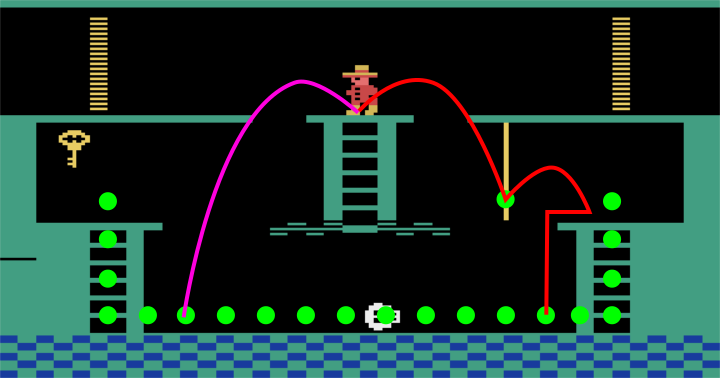
\includegraphics[width=\textwidth / 5 * 3]{img/shaping-defeated.pdf}
\end{center}
\caption{The original shaping rewards, and the two ways the agent found of
  defeating their purpose. First, it took the magenta path. After restricting
  the amount of rewards to be collected at the same time, it took the red
path.\label{fig:shaping-pitfalls}}
\end{figure}

%%% Local Variables: 
%%% mode: latex
%%% TeX-master: "../report"
%%% End: 